\documentclass{standalone}
\usepackage{tikz}
\usetikzlibrary{patterns, positioning}

\begin{document}
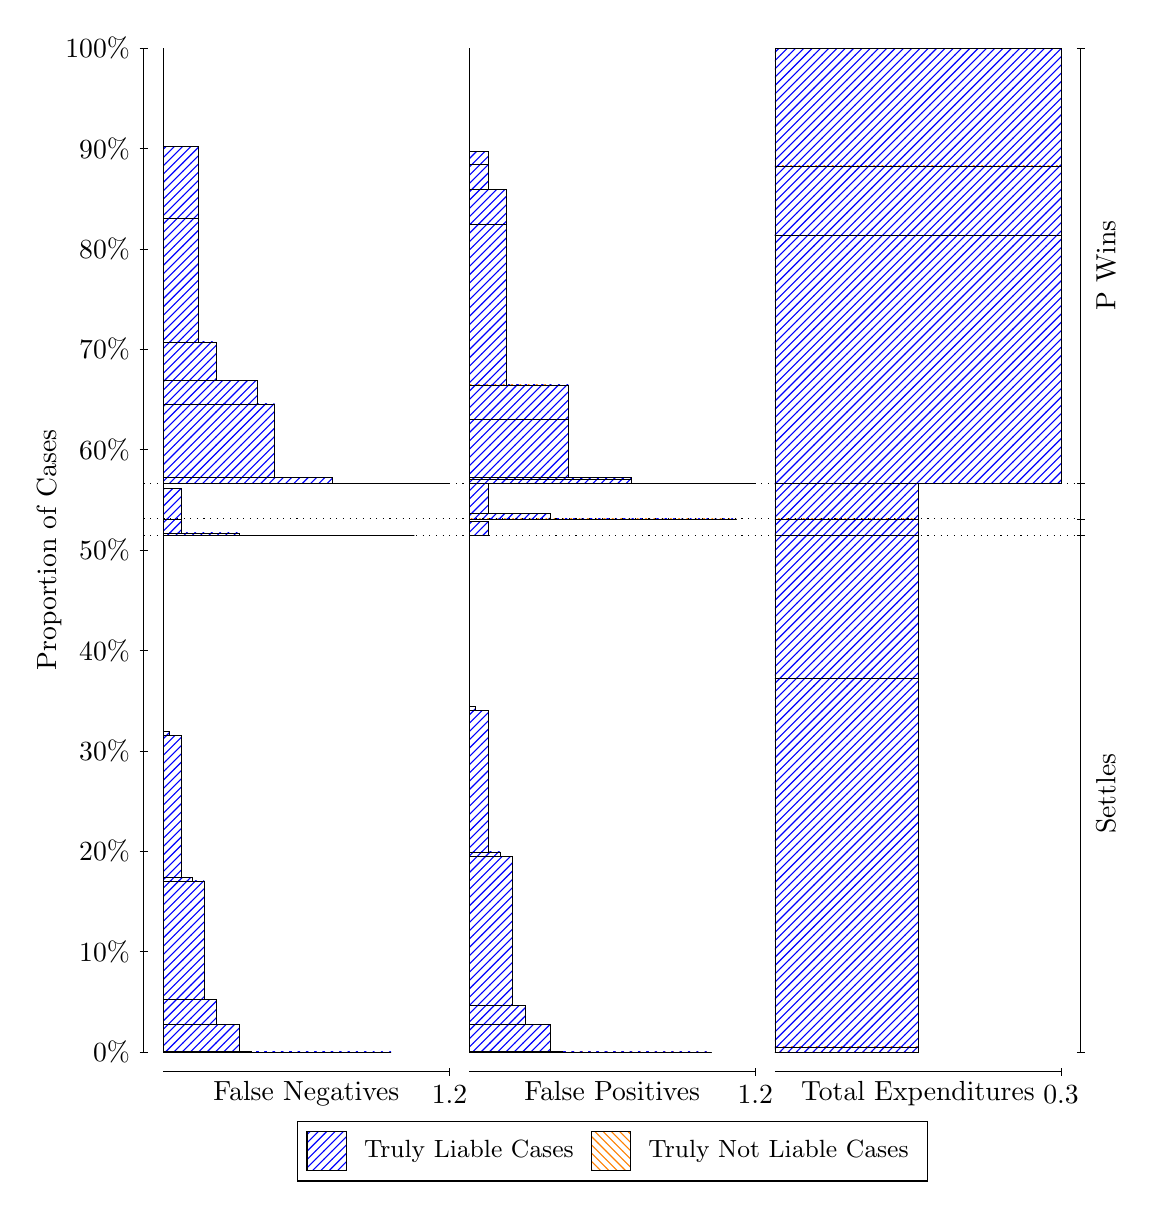
\begin{tikzpicture}
\draw[black, very thin] (1.5,1.75) -- (1.5,14.5);
\node[rotate=90, anchor=center] at (0.3, 8.125) {Proportion of Cases};
\draw[black, very thin] (1.45,1.75) -- (1.55,1.75);
\node[anchor=east] at (1.45, 1.75) {0\%};
\draw[black, very thin] (1.45,3.025) -- (1.55,3.025);
\node[anchor=east] at (1.45, 3.025) {10\%};
\draw[black, very thin] (1.45,4.3) -- (1.55,4.3);
\node[anchor=east] at (1.45, 4.3) {20\%};
\draw[black, very thin] (1.45,5.575) -- (1.55,5.575);
\node[anchor=east] at (1.45, 5.575) {30\%};
\draw[black, very thin] (1.45,6.85) -- (1.55,6.85);
\node[anchor=east] at (1.45, 6.85) {40\%};
\draw[black, very thin] (1.45,8.125) -- (1.55,8.125);
\node[anchor=east] at (1.45, 8.125) {50\%};
\draw[black, very thin] (1.45,9.4) -- (1.55,9.4);
\node[anchor=east] at (1.45, 9.4) {60\%};
\draw[black, very thin] (1.45,10.675) -- (1.55,10.675);
\node[anchor=east] at (1.45, 10.675) {70\%};
\draw[black, very thin] (1.45,11.95) -- (1.55,11.95);
\node[anchor=east] at (1.45, 11.95) {80\%};
\draw[black, very thin] (1.45,13.225) -- (1.55,13.225);
\node[anchor=east] at (1.45, 13.225) {90\%};
\draw[black, very thin] (1.45,14.5) -- (1.55,14.5);
\node[anchor=east] at (1.45, 14.5) {100\%};

\draw[black, very thin] (13.4,1.75) -- (13.4,14.5);
\draw[black, very thin] (13.35,1.75) -- (13.45,1.75);
\node[anchor=west] at (13.35, 1.75) {};
\draw[black, very thin] (13.35,8.3088) -- (13.45,8.3088);
\node[anchor=west] at (13.35, 8.3088) {};
\draw[black, very thin] (13.35,8.521) -- (13.45,8.521);
\node[anchor=west] at (13.35, 8.521) {};
\draw[black, very thin] (13.35,8.9716) -- (13.45,8.9716);
\node[anchor=west] at (13.35, 8.9716) {};
\draw[black, very thin] (13.35,14.5) -- (13.45,14.5);
\node[anchor=west] at (13.35, 14.5) {};

\draw[black, very thin, pattern color=blue, pattern=north east lines] (1.75,1.75) rectangle (4.6418,1.75);
\draw[black, very thin, pattern color=blue, pattern=north east lines] (1.75,1.75) rectangle (4.3452,1.75);
\draw[black, very thin, pattern color=blue, pattern=north east lines] (1.75,1.75) rectangle (4.0486,1.75);
\draw[black, very thin, pattern color=blue, pattern=north east lines] (1.75,1.75) rectangle (3.9003,1.75);
\draw[black, very thin, pattern color=blue, pattern=north east lines] (1.75,1.75) rectangle (3.752,1.75);
\draw[black, very thin, pattern color=blue, pattern=north east lines] (1.75,1.75) rectangle (3.6037,1.75);
\draw[black, very thin, pattern color=blue, pattern=north east lines] (1.75,1.75) rectangle (3.4554,1.751);
\draw[black, very thin, pattern color=blue, pattern=north east lines] (1.75,1.751) rectangle (3.3071,1.751);
\draw[black, very thin, pattern color=blue, pattern=north east lines] (1.75,1.751) rectangle (3.1588,1.7517);
\draw[black, very thin, pattern color=blue, pattern=north east lines] (1.75,1.7517) rectangle (3.0105,1.7517);
\draw[black, very thin, pattern color=blue, pattern=north east lines] (1.75,1.7517) rectangle (3.0105,1.7517);
\draw[black, very thin, pattern color=blue, pattern=north east lines] (1.75,1.7517) rectangle (2.8622,1.7542);
\draw[black, very thin, pattern color=blue, pattern=north east lines] (1.75,1.7542) rectangle (2.7139,2.0993);
\draw[black, very thin, pattern color=blue, pattern=north east lines] (1.75,2.0993) rectangle (2.5656,2.1019);
\draw[black, very thin, pattern color=blue, pattern=north east lines] (1.75,2.1019) rectangle (2.5656,2.1019);
\draw[black, very thin, pattern color=blue, pattern=north east lines] (1.75,2.1019) rectangle (2.4173,2.4149);
\draw[black, very thin, pattern color=blue, pattern=north east lines] (1.75,2.4149) rectangle (2.269,2.4149);
\draw[black, very thin, pattern color=blue, pattern=north east lines] (1.75,2.4149) rectangle (2.269,2.4149);
\draw[black, very thin, pattern color=blue, pattern=north east lines] (1.75,2.4149) rectangle (2.269,3.9217);
\draw[black, very thin, pattern color=blue, pattern=north east lines] (1.75,3.9217) rectangle (2.1207,3.9683);
\draw[black, very thin, pattern color=blue, pattern=north east lines] (1.75,3.9683) rectangle (1.9724,5.7678);
\draw[black, very thin, pattern color=blue, pattern=north east lines] (1.75,5.7678) rectangle (1.8241,5.8261);
\draw[black, very thin, pattern color=blue, pattern=north east lines] (1.75,5.8261) rectangle (1.8241,5.8261);
\draw[black, very thin, pattern color=orange, pattern=north west lines] (1.75,5.8261) rectangle (1.75,5.8261);
\draw[black, very thin, pattern color=blue, pattern=north east lines] (1.75,5.8261) rectangle (1.75,8.3088);
\draw[black, very thin, pattern color=blue, pattern=north east lines] (1.75,8.3088) rectangle (4.9384,8.3088);
\draw[black, very thin, pattern color=blue, pattern=north east lines] (1.75,8.3088) rectangle (4.1969,8.3088);
\draw[black, very thin, pattern color=blue, pattern=north east lines] (1.75,8.3088) rectangle (3.4554,8.3089);
\draw[black, very thin, pattern color=blue, pattern=north east lines] (1.75,8.3089) rectangle (2.7139,8.3412);
\draw[black, very thin, pattern color=blue, pattern=north east lines] (1.75,8.3412) rectangle (1.9724,8.521);
\draw[black, very thin, pattern color=orange, pattern=north west lines] (1.75,8.521) rectangle (1.75,8.521);
\draw[black, very thin, pattern color=blue, pattern=north east lines] (1.75,8.521) rectangle (1.9724,8.9031);
\draw[black, very thin, pattern color=orange, pattern=north west lines] (1.75,8.9031) rectangle (1.75,8.9031);
\draw[black, very thin, pattern color=blue, pattern=north east lines] (1.75,8.9031) rectangle (1.75,8.9716);
\draw[black, very thin, pattern color=blue, pattern=north east lines] (1.75,8.9716) rectangle (5.3833,8.9716);
\draw[black, very thin, pattern color=blue, pattern=north east lines] (1.75,8.9716) rectangle (4.6418,8.9728);
\draw[black, very thin, pattern color=blue, pattern=north east lines] (1.75,8.9728) rectangle (4.4194,8.9728);
\draw[black, very thin, pattern color=blue, pattern=north east lines] (1.75,8.9728) rectangle (3.9003,9.0482);
\draw[black, very thin, pattern color=blue, pattern=north east lines] (1.75,9.0482) rectangle (3.6779,9.0511);
\draw[black, very thin, pattern color=blue, pattern=north east lines] (1.75,9.0511) rectangle (3.1588,9.9817);
\draw[black, very thin, pattern color=blue, pattern=north east lines] (1.75,9.9817) rectangle (2.9364,10.282);
\draw[black, very thin, pattern color=blue, pattern=north east lines] (1.75,10.282) rectangle (2.4173,10.768);
\draw[black, very thin, pattern color=blue, pattern=north east lines] (1.75,10.768) rectangle (2.1949,12.335);
\draw[black, very thin, pattern color=blue, pattern=north east lines] (1.75,12.335) rectangle (2.1949,13.251);
\draw[black, very thin, pattern color=orange, pattern=north west lines] (1.75,13.251) rectangle (1.75,13.251);
\draw[black, very thin, pattern color=blue, pattern=north east lines] (1.75,13.251) rectangle (1.75,14.5);
\draw[black, very thin, pattern color=orange, pattern=north west lines] (5.6333,1.75) rectangle (8.7138,1.75);
\draw[black, very thin, pattern color=blue, pattern=north east lines] (5.6333,1.75) rectangle (8.7138,1.75);
\draw[black, very thin, pattern color=orange, pattern=north west lines] (5.6333,1.75) rectangle (8.3978,1.75);
\draw[black, very thin, pattern color=blue, pattern=north east lines] (5.6333,1.75) rectangle (8.3978,1.75);
\draw[black, very thin, pattern color=orange, pattern=north west lines] (5.6333,1.75) rectangle (8.0819,1.75);
\draw[black, very thin, pattern color=blue, pattern=north east lines] (5.6333,1.75) rectangle (8.0819,1.75);
\draw[black, very thin, pattern color=blue, pattern=north east lines] (5.6333,1.75) rectangle (7.9239,1.75);
\draw[black, very thin, pattern color=orange, pattern=north west lines] (5.6333,1.75) rectangle (7.7659,1.75);
\draw[black, very thin, pattern color=blue, pattern=north east lines] (5.6333,1.75) rectangle (7.7659,1.75);
\draw[black, very thin, pattern color=blue, pattern=north east lines] (5.6333,1.75) rectangle (7.608,1.75);
\draw[black, very thin, pattern color=orange, pattern=north west lines] (5.6333,1.75) rectangle (7.45,1.75);
\draw[black, very thin, pattern color=blue, pattern=north east lines] (5.6333,1.75) rectangle (7.45,1.7508);
\draw[black, very thin, pattern color=blue, pattern=north east lines] (5.6333,1.7508) rectangle (7.292,1.7508);
\draw[black, very thin, pattern color=orange, pattern=north west lines] (5.6333,1.7508) rectangle (7.1341,1.7508);
\draw[black, very thin, pattern color=blue, pattern=north east lines] (5.6333,1.7508) rectangle (7.1341,1.7509);
\draw[black, very thin, pattern color=orange, pattern=north west lines] (5.6333,1.7509) rectangle (7.1341,1.7509);
\draw[black, very thin, pattern color=blue, pattern=north east lines] (5.6333,1.7509) rectangle (7.1341,1.7513);
\draw[black, very thin, pattern color=blue, pattern=north east lines] (5.6333,1.7513) rectangle (6.9761,1.7513);
\draw[black, very thin, pattern color=orange, pattern=north west lines] (5.6333,1.7513) rectangle (6.8181,1.7513);
\draw[black, very thin, pattern color=blue, pattern=north east lines] (5.6333,1.7513) rectangle (6.8181,1.7543);
\draw[black, very thin, pattern color=blue, pattern=north east lines] (5.6333,1.7543) rectangle (6.6601,2.0965);
\draw[black, very thin, pattern color=orange, pattern=north west lines] (5.6333,2.0965) rectangle (6.5022,2.0965);
\draw[black, very thin, pattern color=blue, pattern=north east lines] (5.6333,2.0965) rectangle (6.5022,2.0965);
\draw[black, very thin, pattern color=blue, pattern=north east lines] (5.6333,2.0965) rectangle (6.5022,2.0986);
\draw[black, very thin, pattern color=blue, pattern=north east lines] (5.6333,2.0986) rectangle (6.3442,2.0999);
\draw[black, very thin, pattern color=blue, pattern=north east lines] (5.6333,2.0999) rectangle (6.3442,2.3463);
\draw[black, very thin, pattern color=orange, pattern=north west lines] (5.6333,2.3463) rectangle (6.1862,2.3463);
\draw[black, very thin, pattern color=blue, pattern=north east lines] (5.6333,2.3463) rectangle (6.1862,4.2325);
\draw[black, very thin, pattern color=blue, pattern=north east lines] (5.6333,4.2325) rectangle (6.1862,4.2327);
\draw[black, very thin, pattern color=blue, pattern=north east lines] (5.6333,4.2327) rectangle (6.0283,4.2909);
\draw[black, very thin, pattern color=blue, pattern=north east lines] (5.6333,4.2909) rectangle (5.8703,6.0905);
\draw[black, very thin, pattern color=blue, pattern=north east lines] (5.6333,6.0905) rectangle (5.7123,6.0905);
\draw[black, very thin, pattern color=blue, pattern=north east lines] (5.6333,6.0905) rectangle (5.7123,6.137);
\draw[black, very thin, pattern color=blue, pattern=north east lines] (5.6333,6.137) rectangle (5.6333,8.3088);
\draw[black, very thin, pattern color=orange, pattern=north west lines] (5.6333,8.3088) rectangle (5.8703,8.3088);
\draw[black, very thin, pattern color=blue, pattern=north east lines] (5.6333,8.3088) rectangle (5.8703,8.4886);
\draw[black, very thin, pattern color=blue, pattern=north east lines] (5.6333,8.4886) rectangle (5.6333,8.521);
\draw[black, very thin, pattern color=orange, pattern=north west lines] (5.6333,8.521) rectangle (9.0297,8.521);
\draw[black, very thin, pattern color=blue, pattern=north east lines] (5.6333,8.521) rectangle (9.0297,8.521);
\draw[black, very thin, pattern color=blue, pattern=north east lines] (5.6333,8.521) rectangle (8.2399,8.521);
\draw[black, very thin, pattern color=blue, pattern=north east lines] (5.6333,8.521) rectangle (7.45,8.5214);
\draw[black, very thin, pattern color=blue, pattern=north east lines] (5.6333,8.5214) rectangle (6.6601,8.5895);
\draw[black, very thin, pattern color=blue, pattern=north east lines] (5.6333,8.5895) rectangle (5.8703,8.9716);
\draw[black, very thin, pattern color=orange, pattern=north west lines] (5.6333,8.9716) rectangle (9.2667,8.9716);
\draw[black, very thin, pattern color=blue, pattern=north east lines] (5.6333,8.9716) rectangle (9.2667,8.9716);
\draw[black, very thin, pattern color=orange, pattern=north west lines] (5.6333,8.9716) rectangle (8.4768,8.9716);
\draw[black, very thin, pattern color=blue, pattern=north east lines] (5.6333,8.9716) rectangle (8.4768,8.9719);
\draw[black, very thin, pattern color=blue, pattern=north east lines] (5.6333,8.9719) rectangle (8.4768,8.9727);
\draw[black, very thin, pattern color=orange, pattern=north west lines] (5.6333,8.9727) rectangle (7.687,8.9727);
\draw[black, very thin, pattern color=blue, pattern=north east lines] (5.6333,8.9727) rectangle (7.687,9.0283);
\draw[black, very thin, pattern color=blue, pattern=north east lines] (5.6333,9.0283) rectangle (7.687,9.045);
\draw[black, very thin, pattern color=orange, pattern=north west lines] (5.6333,9.045) rectangle (7.45,9.045);
\draw[black, very thin, pattern color=blue, pattern=north east lines] (5.6333,9.045) rectangle (7.45,9.045);
\draw[black, very thin, pattern color=orange, pattern=north west lines] (5.6333,9.045) rectangle (6.8971,9.045);
\draw[black, very thin, pattern color=blue, pattern=north east lines] (5.6333,9.045) rectangle (6.8971,9.7884);
\draw[black, very thin, pattern color=blue, pattern=north east lines] (5.6333,9.7884) rectangle (6.8971,10.221);
\draw[black, very thin, pattern color=orange, pattern=north west lines] (5.6333,10.221) rectangle (6.6601,10.221);
\draw[black, very thin, pattern color=blue, pattern=north east lines] (5.6333,10.221) rectangle (6.6601,10.221);
\draw[black, very thin, pattern color=blue, pattern=north east lines] (5.6333,10.221) rectangle (6.6601,10.221);
\draw[black, very thin, pattern color=blue, pattern=north east lines] (5.6333,10.221) rectangle (6.1072,12.268);
\draw[black, very thin, pattern color=blue, pattern=north east lines] (5.6333,12.268) rectangle (6.1072,12.704);
\draw[black, very thin, pattern color=blue, pattern=north east lines] (5.6333,12.704) rectangle (5.8703,12.704);
\draw[black, very thin, pattern color=orange, pattern=north west lines] (5.6333,12.704) rectangle (5.8703,12.704);
\draw[black, very thin, pattern color=blue, pattern=north east lines] (5.6333,12.704) rectangle (5.8703,13.022);
\draw[black, very thin, pattern color=blue, pattern=north east lines] (5.6333,13.022) rectangle (5.8703,13.19);
\draw[black, very thin, pattern color=blue, pattern=north east lines] (5.6333,13.19) rectangle (5.6333,14.5);
\draw[black, very thin, pattern color=orange, pattern=north west lines] (9.5167,1.75) rectangle (11.333,1.75);
\draw[black, very thin, pattern color=blue, pattern=north east lines] (9.5167,1.75) rectangle (11.333,1.8154);
\draw[black, very thin, pattern color=orange, pattern=north west lines] (9.5167,1.8154) rectangle (11.333,1.8154);
\draw[black, very thin, pattern color=blue, pattern=north east lines] (9.5167,1.8154) rectangle (11.333,6.4991);
\draw[black, very thin, pattern color=orange, pattern=north west lines] (9.5167,6.4991) rectangle (11.333,6.4991);
\draw[black, very thin, pattern color=blue, pattern=north east lines] (9.5167,6.4991) rectangle (11.333,8.3088);
\draw[black, very thin, pattern color=orange, pattern=north west lines] (9.5167,8.3088) rectangle (11.333,8.3088);
\draw[black, very thin, pattern color=blue, pattern=north east lines] (9.5167,8.3088) rectangle (11.333,8.521);
\draw[black, very thin, pattern color=orange, pattern=north west lines] (9.5167,8.521) rectangle (11.333,8.521);
\draw[black, very thin, pattern color=blue, pattern=north east lines] (9.5167,8.521) rectangle (11.333,8.9716);
\draw[black, very thin, pattern color=orange, pattern=north west lines] (9.5167,8.9716) rectangle (13.15,8.9716);
\draw[black, very thin, pattern color=blue, pattern=north east lines] (9.5167,8.9716) rectangle (13.15,12.121);
\draw[black, very thin, pattern color=orange, pattern=north west lines] (9.5167,12.121) rectangle (13.15,12.121);
\draw[black, very thin, pattern color=blue, pattern=north east lines] (9.5167,12.121) rectangle (13.15,13.002);
\draw[black, very thin, pattern color=orange, pattern=north west lines] (9.5167,13.002) rectangle (13.15,13.002);
\draw[black, very thin, pattern color=blue, pattern=north east lines] (9.5167,13.002) rectangle (13.15,14.5);
\draw[black, dotted] (1.5,8.3088) -- (13.4,8.3088);
\draw[black, dotted] (1.5,8.521) -- (13.4,8.521);
\draw[black, dotted] (1.5,8.9716) -- (13.4,8.9716);
\draw[black, very thin] (1.75,1.5) -- (5.3833,1.5);
\node[anchor=north] at (3.5667, 1.5) {False Negatives};
\draw[black, very thin] (5.3833,1.45) -- (5.3833,1.55);
\node[anchor=north] at (5.3833, 1.45) {1.2};

\draw[black, very thin] (5.6333,1.5) -- (9.2667,1.5);
\node[anchor=north] at (7.45, 1.5) {False Positives};
\draw[black, very thin] (9.2667,1.45) -- (9.2667,1.55);
\node[anchor=north] at (9.2667, 1.45) {1.2};

\draw[black, very thin] (9.5167,1.5) -- (13.15,1.5);
\node[anchor=north] at (11.333, 1.5) {Total Expenditures};
\draw[black, very thin] (13.15,1.45) -- (13.15,1.55);
\node[anchor=north] at (13.15, 1.45) {0.3};

\node[black, centered, rotate=90] at (13.72, 5.0294) {Settles};


\node[black, centered, rotate=90] at (13.72, 11.736) {P Wins};

\draw (7.449999999999999,1.5) node[draw=none] (baseCoordinate) {};
\begin{scope}[align=center]
        \matrix[scale=0.5, draw=black, below=0.5cm of baseCoordinate, nodes={draw}, column sep=0.1cm]{
            \node[rectangle, draw, minimum width=0.5cm, minimum height=0.5cm, pattern=north east lines, pattern color=blue] {}; &
            \node[draw=none, font=\small] (B) {Truly Liable Cases}; &
            \node[rectangle, draw, minimum width=0.5cm, minimum height=0.5cm, pattern=north west lines, pattern color=orange] {}; &
            \node[draw=none, font=\small] (B) {Truly Not Liable Cases}; \\
            };
\end{scope}

\end{tikzpicture}
\end{document}